\documentclass[dvipdfmx]{jsarticle} %A4: 21.0 x 29.7cm
\usepackage{amsmath,amsfonts,amssymb,amsthm}
\usepackage{mathtools}
\usepackage{xcolor}
\usepackage{otf}
\usepackage{xspace}
\usepackage{newpxtext}
\usepackage{tikz}
\usetikzlibrary{positioning, arrows.meta}
\renewcommand{\abstractname}{注意事項}
% \renewcommand{\qed}{\unskip\nobreak\quad\qedsymbol}
\newtagform{textbf}[\textbf]{[}{]}
\usetagform{textbf}
\newcommand*{\ie}{\textbf{\textit{i.e.}}\@\xspace}
\renewcommand{\qedsymbol}{$\blacksquare$}


\title{\vspace{-4cm}確率過程論のレポート問題}
\author{\texttt{YI\ Ran} - $\mathnormal{21122200512}$\\ \texttt{andreyi@outlook.jp}}
\date{\today}

\begin{document}
\maketitle


\begin{abstract}
  \textcolor{red}{A4で1枚にまとめること、提出は07月03日(13回)か07月10日(14回)のいずれかの授業中}  
\end{abstract}
\section*{問題}
$ \sigma_3 \left(\left\{0\right\}, \left\{-3,1\right\}\right) $を確率的手法と格子グラフ的手法のそれぞれにより求めよ。
\vspace{-0.4cm}
\section*{解答}
\begin{proof}[\textbf{proof}]
(確率的手法)
\begin{figure}[htbp]
$ \sigma_3 \left(\left\{0\right\}, \left\{-3,1\right\}\right) $を確率的手法で求めると、以下のようになります。\\[1em]

   \begin{tikzpicture} 
% 原始三角形
\draw[line width=0.5pt, rounded corners=8pt, black] 
    (0,0) -- (0,1) -- (0.87,0.5) -- cycle;
\draw[fill=black, draw=black, line width=0.5pt] (0.13,0.22) node[left=0.2em]{\small 0} circle (2pt);
\draw[fill=white, draw=black, line width=0.5pt] (0.13,0.78) node[left=0.2em]{\small 2} node[above right=1.5em]{\small 図1} node[above=5em]{\small 「$\circ=0$, $\bullet=1$」を表す} circle (2pt);
\draw[fill=white, draw=black, line width=0.5pt] (0.61,0.5) node[left=0.05em]{\small $1$-$p$} circle (2pt);

% 向右平移3个单位,向上平移2个单位
\begin{scope}[shift={(0,-0.56)}]
    \draw[line width=0.5pt, rounded corners=8pt, black] 
          (0,0) -- (0,1) -- (0.87,0.5) -- cycle;
    \draw[fill=white, draw=black, line width=0.5pt] (0.13,0.22) node[left=0.2em]{\small -2} circle (2pt);
    % \draw[fill=white, draw=black, line width=0.5pt] (4.7,0.2) node[left=0.5em]{-2} circle (3pt);
    \draw[fill=black, draw=black, line width=0.5pt] (0.61,0.5) node[left=0.2em]{\small $p$} circle (2pt);
\end{scope}
\begin{scope}[shift={(0.48,-0.28)}]
    \draw[line width=0.5pt, rounded corners=8pt, black] 
          (0,0) -- (0,1) -- (0.87,0.5) -- cycle;
    % \draw[fill=black, draw=black, line width=0.5pt] (3.3,0.2) circle (3pt);
    % \draw[fill=black, draw=black, line width=0.5pt] (4.7,0.2) circle (3pt);
    \draw[fill=black, draw=black, line width=0.5pt] (0.61,0.5) node[left=0.2em]{\small $p$} circle (2pt);
\end{scope}
\begin{scope}[shift={(0.48,-0.84)}]
    \draw[line width=0.5pt, rounded corners=8pt, black] 
          (0,0) -- (0,1) -- (0.87,0.5) -- cycle;
    \draw[fill=white, draw=black, line width=0.5pt] (0.13,0.22) circle (2pt);
    % \draw[fill=black, draw=black, line width=0.5pt] (4.7,0.2) circle (3pt);
    \draw[fill=black, draw=black, line width=0.5pt] (0.61,0.5) node[left=0.2em]{\small $p$} circle (2pt);
\end{scope}
\begin{scope}[shift={(0.96,-0.01)}]
    \draw[line width=0.5pt, rounded corners=8pt, black] 
          (0,0) -- (0,1) -- (0.87,0.5) -- cycle;
    % \draw[fill=white, draw=black, line width=0.5pt] (0.13,0.22) circle (2pt);
    \draw[fill=white, draw=black, line width=0.5pt] (0.13,0.78) circle (2pt);
    \draw[fill=black, draw=black, line width=0.5pt] (0.61,0.5) node[right=0.2em]{\small 1} node[left=0.2em]{\small $p$} circle (2pt);
\end{scope}
\begin{scope}[shift={(0.96,-1.11)}]
    \draw[line width=0.5pt, rounded corners=8pt, black] 
          (0,0) -- (0,1) -- (0.87,0.5) -- cycle;
    \draw[fill=white, draw=black, line width=0.5pt] (0.13,0.22) circle (2pt);
    % \draw[fill=white, draw=black, line width=0.5pt] (0.13,0.78) circle (2pt);
    \draw[fill=black, draw=black, line width=0.5pt] (0.61,0.5) node[right=0.2em]{\small -3} node[left=0.2em]{\small $p$} circle (2pt);
\end{scope}


  
% \end{scope}
\draw[stealth-stealth, thick] (-1,-1) -- (-1,1.6) node[left=0.4em] at (-1,0.5) {\small \shortstack{空\\間}};
\draw[stealth-stealth, thick] (-1,-1.4) -- (2.5,-1.4) node[below=1.5em] at (0.9,-1.3) {\small 時\ 間};

% 手动指定每个刻度的位置和标签
\draw[thick] (0.1,-1.3) -- (0.1,-1.5) node[below] {\small 0};
\draw[thick] (0.6,-1.3) -- (0.6,-1.5) node[below] {\small 1};
\draw[thick] (1.1,-1.3) -- (1.1,-1.5) node[below] {\small 2};
\draw[thick] (1.6,-1.3) -- (1.6,-1.5) node[below] {\small 3};
%図2
\begin{scope}[shift={(3.5,-0.56)}]
    \draw[line width=0.5pt, rounded corners=8pt, black] 
          (0,0) -- (0,1) -- (0.87,0.5) -- cycle;
    \draw[fill=white, draw=black, line width=0.5pt] (0.13,0.22) node[left=0.2em]{\small -2} circle (2pt);
    % \draw[fill=white, draw=black, line width=0.5pt] (4.7,0.2) node[left=0.5em]{-2} circle (3pt);
    \draw[fill=black, draw=black, line width=0.5pt] (0.61,0.5) node[left=0.2em]{\small $p$} circle (2pt);
\end{scope}
\begin{scope}[shift={(3.5,0.005)}]
    \draw[line width=0.5pt, rounded corners=8pt, black] 
          (0,0) -- (0,1) -- (0.87,0.5) -- cycle;
    \draw[fill=black, draw=black, line width=0.5pt] (0.13,0.22) node[left=0.2em]{\small 0} circle (2pt);
    \draw[fill=white, draw=black, line width=0.5pt] (0.13,0.78) node[left=0.2em]{\small 2} circle (2pt);
    \draw[fill=black, draw=black, line width=0.5pt] (0.61,0.5) node[left=0.2em]{\small $p$} circle (2pt);
\end{scope}
\begin{scope}[shift={(3.98,-0.277)}]
    \draw[line width=0.5pt, rounded corners=8pt, black] 
          (0,0) -- (0,1) -- (0.87,0.5) -- cycle;
    % \draw[fill=white, draw=black, line width=0.5pt] (0.13,0.22) node[left=0.2em]{\small -2} circle (2pt);
    % \draw[fill=white, draw=black, line width=0.5pt] (0.13,0.78) circle (2pt);
    \draw[fill=white, draw=black, line width=0.5pt] (0.61,0.5) node[left=0.01em]{\footnotesize $1$-$q$} circle (2pt);
\end{scope}
\begin{scope}[shift={(3.98,0.28)}]
    \draw[line width=0.5pt, rounded corners=8pt, black] 
          (0,0) -- (0,1) -- (0.87,0.5) -- cycle;
    %\draw[fill=white, draw=black, line width=0.5pt] (0.13,0.22) node[left=0.2em]{\small -2} circle (2pt);
    \draw[fill=white, draw=black, line width=0.5pt] (0.13,0.78) node[above=0.3em]{\small 図2} circle (2pt);
    \draw[fill=black, draw=black, line width=0.5pt] (0.61,0.5) node[left=0.2em]{\small $p$} circle (2pt);
\end{scope}
\begin{scope}[shift={(3.98,-0.84)}]
    \draw[line width=0.5pt, rounded corners=8pt, black] 
          (0,0) -- (0,1) -- (0.87,0.5) -- cycle;
    \draw[fill=white, draw=black, line width=0.5pt] (0.13,0.22)  circle (2pt);
    % \draw[fill=white, draw=black, line width=0.5pt] (0.13,0.78) circle (2pt);
    \draw[fill=black, draw=black, line width=0.5pt] (0.61,0.5) node[left=0.2em]{\small $p$} circle (2pt);
\end{scope}
\begin{scope}[shift={(4.46,-0.001)}]
    \draw[line width=0.5pt, rounded corners=8pt, black] 
          (0,0) -- (0,1) -- (0.87,0.5) -- cycle;
    % \draw[fill=white, draw=black, line width=0.5pt] (0.13,0.22) node[left=0.2em]{\small -2} circle (2pt);
    % \draw[fill=white, draw=black, line width=0.5pt] (0.13,0.78) circle (2pt);
    \draw[fill=black, draw=black, line width=0.5pt] (0.61,0.5) node[right=0.2em]{\small 1} node[left=0.2em]{\small $p$} circle (2pt);
\end{scope}
\begin{scope}[shift={(4.46,-1.12)}]
    \draw[line width=0.5pt, rounded corners=8pt, black] 
          (0,0) -- (0,1) -- (0.87,0.5) -- cycle;
    \draw[fill=white, draw=black, line width=0.5pt] (0.13,0.22)  circle (2pt);
    % \draw[fill=white, draw=black, line width=0.5pt] (0.13,0.78) circle (2pt);
    \draw[fill=black, draw=black, line width=0.5pt] (0.61,0.5) node[right=0.2em]{\small -3} node[left=0.2em]{\small $p$} circle (2pt);
\end{scope}
%図3
\begin{scope}[shift={(7,-0.56)}]
    \draw[line width=0.5pt, rounded corners=8pt, black] 
          (0,0) -- (0,1) -- (0.87,0.5) -- cycle;
    \draw[fill=white, draw=black, line width=0.5pt] (0.13,0.22) node[left=0.2em]{\small -2} circle (2pt);
    % \draw[fill=white, draw=black, line width=0.5pt] (4.7,0.2) node[left=0.5em]{-2} circle (3pt);
    \draw[fill=black, draw=black, line width=0.5pt] (0.61,0.5) node[left=0.2em]{\small $p$} circle (2pt);
\end{scope}
\begin{scope}[shift={(7,0.005)}]
    \draw[line width=0.5pt, rounded corners=8pt, black] 
          (0,0) -- (0,1) -- (0.87,0.5) -- cycle;
    \draw[fill=black, draw=black, line width=0.5pt] (0.13,0.22) node[left=0.2em]{\small 0} circle (2pt);
    \draw[fill=white, draw=black, line width=0.5pt] (0.13,0.78) node[left=0.2em]{\small 2} circle (2pt);
    \draw[fill=black, draw=black, line width=0.5pt] (0.61,0.5) node[left=0.2em]{\small $p$} circle (2pt);
\end{scope}
\begin{scope}[shift={(7.48,-0.277)}]
    \draw[line width=0.5pt, rounded corners=8pt, black] 
          (0,0) -- (0,1) -- (0.87,0.5) -- cycle;
    % \draw[fill=white, draw=black, line width=0.5pt] (0.13,0.22) node[left=0.2em]{\small -2} circle (2pt);
    % \draw[fill=white, draw=black, line width=0.5pt] (0.13,0.78) circle (2pt);
    \draw[fill=black, draw=black, line width=0.5pt] (0.61,0.5) node[left=0.01em]{\small $q$} circle (2pt);
\end{scope}
\begin{scope}[shift={(7.48,0.28)}]
    \draw[line width=0.5pt, rounded corners=8pt, black] 
          (0,0) -- (0,1) -- (0.87,0.5) -- cycle;
    %\draw[fill=white, draw=black, line width=0.5pt] (0.13,0.22) node[left=0.2em]{\small -2} circle (2pt);
    \draw[fill=white, draw=black, line width=0.5pt] (0.13,0.78) node[above=0.3em]{\small 図3} circle (2pt);
    \draw[fill=white, draw=black, line width=0.5pt] (0.61,0.5) node[left=0.05em]{\small $1$-$p$} circle (2pt);
\end{scope}
\begin{scope}[shift={(7.48,-0.84)}]
    \draw[line width=0.5pt, rounded corners=8pt, black] 
          (0,0) -- (0,1) -- (0.87,0.5) -- cycle;
    \draw[fill=white, draw=black, line width=0.5pt] (0.13,0.22)  circle (2pt);
    % \draw[fill=white, draw=black, line width=0.5pt] (0.13,0.78) circle (2pt);
    \draw[fill=black, draw=black, line width=0.5pt] (0.61,0.5) node[left=0.2em]{\small $p$} circle (2pt);
\end{scope}
\begin{scope}[shift={(7.96,-0.001)}]
    \draw[line width=0.5pt, rounded corners=8pt, black] 
          (0,0) -- (0,1) -- (0.87,0.5) -- cycle;
    % \draw[fill=white, draw=black, line width=0.5pt] (0.13,0.22) node[left=0.2em]{\small -2} circle (2pt);
    % \draw[fill=white, draw=black, line width=0.5pt] (0.13,0.78) circle (2pt);
    \draw[fill=black, draw=black, line width=0.5pt] (0.61,0.5) node[right=0.2em]{\small 1} node[left=0.2em]{\small $p$} circle (2pt);
\end{scope}
\begin{scope}[shift={(7.96,-1.12)}]
    \draw[line width=0.5pt, rounded corners=8pt, black] 
          (0,0) -- (0,1) -- (0.87,0.5) -- cycle;
    \draw[fill=white, draw=black, line width=0.5pt] (0.13,0.22)  circle (2pt);
    % \draw[fill=white, draw=black, line width=0.5pt] (0.13,0.78) circle (2pt);
    \draw[fill=black, draw=black, line width=0.5pt] (0.61,0.5) node[right=0.2em]{\small -3} node[left=0.2em]{\small $p$} circle (2pt);
\end{scope}
%図4
\begin{scope}[shift={(10.5,-0.56)}]
    \draw[line width=0.5pt, rounded corners=8pt, black] 
          (0,0) -- (0,1) -- (0.87,0.5) -- cycle;
    \draw[fill=white, draw=black, line width=0.5pt] (0.13,0.22) node[left=0.2em]{\small -2} circle (2pt);
    % \draw[fill=white, draw=black, line width=0.5pt] (4.7,0.2) node[left=0.5em]{-2} circle (3pt);
    \draw[fill=black, draw=black, line width=0.5pt] (0.61,0.5) node[left=0.2em]{\small $p$} circle (2pt);
\end{scope}
\begin{scope}[shift={(10.5,0.005)}]
    \draw[line width=0.5pt, rounded corners=8pt, black] 
          (0,0) -- (0,1) -- (0.87,0.5) -- cycle;
    \draw[fill=black, draw=black, line width=0.5pt] (0.13,0.22) node[left=0.2em]{\small 0} circle (2pt);
    \draw[fill=white, draw=black, line width=0.5pt] (0.13,0.78) node[left=0.2em]{\small 2} circle (2pt);
    \draw[fill=black, draw=black, line width=0.5pt] (0.61,0.5) node[left=0.2em]{\small $p$} circle (2pt);
\end{scope}
\begin{scope}[shift={(10.98,-0.277)}]
    \draw[line width=0.5pt, rounded corners=8pt, black] 
          (0,0) -- (0,1) -- (0.87,0.5) -- cycle;
    % \draw[fill=white, draw=black, line width=0.5pt] (0.13,0.22) node[left=0.2em]{\small -2} circle (2pt);
    % \draw[fill=white, draw=black, line width=0.5pt] (0.13,0.78) circle (2pt);
    \draw[fill=black, draw=black, line width=0.5pt] (0.61,0.5) node[left=0.01em]{\small $q$} circle (2pt);
\end{scope}
\begin{scope}[shift={(10.98,0.28)}]
    \draw[line width=0.5pt, rounded corners=8pt, black] 
          (0,0) -- (0,1) -- (0.87,0.5) -- cycle;
    %\draw[fill=white, draw=black, line width=0.5pt] (0.13,0.22) node[left=0.2em]{\small -2} circle (2pt);
    \draw[fill=white, draw=black, line width=0.5pt] (0.13,0.78) node[above=0.3em]{\small 図4} circle (2pt);
    \draw[fill=black, draw=black, line width=0.5pt] (0.61,0.5) node[left=0.05em]{\small $p$} circle (2pt);
\end{scope}
\begin{scope}[shift={(10.98,-0.84)}]
    \draw[line width=0.5pt, rounded corners=8pt, black] 
          (0,0) -- (0,1) -- (0.87,0.5) -- cycle;
    \draw[fill=white, draw=black, line width=0.5pt] (0.13,0.22)  circle (2pt);
    % \draw[fill=white, draw=black, line width=0.5pt] (0.13,0.78) circle (2pt);
    \draw[fill=black, draw=black, line width=0.5pt] (0.61,0.5) node[left=0.2em]{\small $p$} circle (2pt);
\end{scope}
\begin{scope}[shift={(11.46,-0.001)}]
    \draw[line width=0.5pt, rounded corners=8pt, black] 
          (0,0) -- (0,1) -- (0.87,0.5) -- cycle;
    % \draw[fill=white, draw=black, line width=0.5pt] (0.13,0.22) node[left=0.2em]{\small -2} circle (2pt);
    % \draw[fill=white, draw=black, line width=0.5pt] (0.13,0.78) circle (2pt);
    \draw[fill=black, draw=black, line width=0.5pt] (0.61,0.5) node[right=0.2em]{\small 1} node[left=0.2em]{\small $q$} circle (2pt);
\end{scope}
\begin{scope}[shift={(11.46,-1.12)}]
    \draw[line width=0.5pt, rounded corners=8pt, black] 
          (0,0) -- (0,1) -- (0.87,0.5) -- cycle;
    \draw[fill=white, draw=black, line width=0.5pt] (0.13,0.22) circle (2pt);
    % \draw[fill=white, draw=black, line width=0.5pt] (0.13,0.78) circle (2pt);
    \draw[fill=black, draw=black, line width=0.5pt] (0.61,0.5) node[right=0.2em]{\small -3} node[left=0.2em]{\small $p$} circle (2pt);
\end{scope}
\end{tikzpicture}
\end{figure}

\begin{figure}[htbp]
   
次に、Domany-Kinzelモデルのルールは以下のように表している。\\[1em]
  %Domany-Kinzelモデルのルール
\begin{tikzpicture}
  \draw[line width=0.5pt, rounded corners=8pt, black] 
    (0,0) -- (1,0) -- (0.5,-0.87) -- cycle;
\draw[fill=white, draw=black, line width=0.5pt] (0.22,-0.13)  circle (2pt);
\draw[fill=black, draw=black, line width=0.5pt] (0.5,-0.62) node[below=0.4em]{\footnotesize 確率0}  circle (2pt);
\draw[fill=white, draw=black, line width=0.5pt] (0.78,-0.13)  circle (2pt);

\begin{scope}[shift={(1.5,0)}]
  \draw[line width=0.5pt, rounded corners=8pt, black] 
    (0,0) -- (1,0) -- (0.5,-0.87) -- cycle;
\draw[fill=white, draw=black, line width=0.5pt] (0.22,-0.13)  circle (2pt);
\draw[fill=black, draw=black, line width=0.5pt] (0.5,-0.62) node[below=0.4em]{\footnotesize 確率$p$} circle (2pt);
\draw[fill=black, draw=black, line width=0.5pt] (0.78,-0.13)  circle (2pt);  
  
\end{scope}

\begin{scope}[shift={(3,0)}]
  \draw[line width=0.5pt, rounded corners=8pt, black] 
    (0,0) -- (1,0) -- (0.5,-0.87) -- cycle;
\draw[fill=black, draw=black, line width=0.5pt] (0.22,-0.13) circle (2pt);     
\draw[fill=black, draw=black, line width=0.5pt] (0.5,-0.62) node[below=0.4em]{\footnotesize 確率$p$} circle (2pt);
\draw[fill=white, draw=black, line width=0.5pt] (0.78,-0.13) circle (2pt);    
\end{scope}

\begin{scope}[shift={(4.5,0)}]
  \draw[line width=0.5pt, rounded corners=8pt, black] 
    (0,0) -- (1,0) -- (0.5,-0.87) -- cycle;
\draw[fill=black, draw=black, line width=0.5pt] (0.22,-0.13) circle (2pt);
\draw[fill=black, draw=black, line width=0.5pt] (0.5,-0.62) node[below=0.4em]{\footnotesize 確率$q$} circle (2pt);  
\draw[fill=black, draw=black, line width=0.5pt] (0.78,-0.13) circle (2pt);  
\end{scope}

%下方图形

\begin{scope}[shift={(0,-2)}]
\draw[line width=0.5pt, rounded corners=8pt, black] 
  (0,0) -- (1,0) -- (0.5,-0.87) -- cycle;
\draw[fill=white, draw=black, line width=0.5pt] (0.22,-0.13) circle (2pt);
\draw[fill=white, draw=black, line width=0.5pt] (0.5,-0.62) node[below=0.4em]{\footnotesize 確率1} circle (2pt);
\draw[fill=white, draw=black, line width=0.5pt] (0.78,-0.13)  circle (2pt);
\end{scope}

\begin{scope}[shift={(1.5,-2)}]
\draw[line width=0.5pt, rounded corners=8pt, black] 
  (0,0) -- (1,0) -- (0.5,-0.87) -- cycle;
\draw[fill=white, draw=black, line width=0.5pt] (0.22,-0.13) circle (2pt);
\draw[fill=white, draw=black, line width=0.5pt] (0.5,-0.62) node[below=0.4em]{\footnotesize 確率1-$p$}  circle (2pt);
\draw[fill=black, draw=black, line width=0.5pt] (0.78,-0.13)  circle (2pt);
  
\end{scope}

\begin{scope}[shift={(3,-2)}]
\draw[line width=0.5pt, rounded corners=8pt, black] 
  (0,0) -- (1,0) -- (0.5,-0.87) -- cycle;
\draw[fill=black, draw=black, line width=0.5pt] (0.22,-0.13) circle (2pt);
\draw[fill=white, draw=black, line width=0.5pt] (0.5,-0.62) node[below=0.4em]{\footnotesize 確率1-$p$}  circle (2pt);
\draw[fill=white, draw=black, line width=0.5pt] (0.78,-0.13)  circle (2pt);
  
\end{scope}

\begin{scope}[shift={(4.5,-2)}]
\draw[line width=0.5pt, rounded corners=8pt, black] 
  (0,0) -- (1,0) -- (0.5,-0.87) -- cycle;
\draw[fill=black, draw=black, line width=0.5pt] (0.22,-0.13) circle (2pt);
\draw[fill=white, draw=black, line width=0.5pt] (0.5,-0.62) node[below=0.4em]{\footnotesize 確率1-$q$}  circle (2pt);
\draw[fill=black, draw=black, line width=0.5pt] (0.78,-0.13)  circle (2pt);
  
\end{scope}

\draw[<-, thick] (-0.5,-1) -- (-0.5,0.1) node[left=0.2em] at (-0.5,-0.4) {\small \shortstack{時\\間}};
\draw[<-, thick] (-0.5,-3) -- (-0.5,-2) node[left=0.2em] at (-0.5,-2.4) {\small \shortstack{時\\間}};
\end{tikzpicture}
  
\end{figure}

\ \\
したがって、\\
図1の確率は $ p^5(1-p) $,図2の確率は $ p^6(1-q) $,
図3の確率は $ p^5(1-p)q $,図4の確率は $ p^5 q^2 $ である。\\
\ie\quad $ \sigma_3 \left(\left\{0\right\}, \left\{-3,1\right\}\right) =p^5 \left\{\left(1-p\right)+p\left(1-q\right)+\left(1-p\right)q+q^2\right\}=p^5\left(1+q-2pq+q^2\right)$
\end{proof}
\ \\
\begin{proof}[\textbf{proof}]
(格子グラフ的手法)

\begin{figure}[htbp]
  格子グラフ的手法による$ \sigma_3 \left(\left\{0\right\}, \left\{-3,1\right\}\right)$の導出は以下の図の記号を用いる。\\[1em]
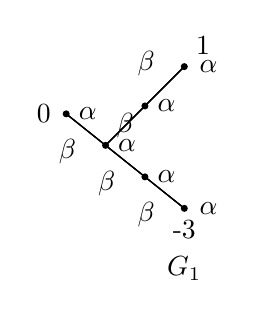
\begin{tikzpicture}
   \draw[line width=0.5pt, rounded corners=8pt, black] 
          (0,0) -- (1.5,-1.2);
  \draw[fill=black, draw=black, line width=0.5pt] (0,0) node[left=0.2em]{0} node[right=0.1em]{$ \alpha $}  circle (1pt);
  % \draw[fill=white, draw=black, line width=0.5pt] (0.13,0.78) circle (2pt);
  \draw[fill=black, draw=black, line width=0.5pt] (1.5,0.6) node[right=0.2em]{$ \alpha $} node[above right=0.1em]{1}  circle (1pt);
  \draw[line width =0.5pt,black]
  (0.5,-0.4) -- (1.5,0.6);
  % \draw[fill=black, draw=black, line width=0.5pt] (0.5,-0.33) circle (1pt);
  \draw[fill=black, draw=black, line width=0.5pt] (1.5,-1.2) node[below=1.4em]{$ G_1 $} node[right=0.2em]{$ \alpha $} node[below=0.1em]{-3} circle (1pt);
  \draw[fill=black, draw=black, line width=0.5pt] (0.5,-0.4) node[right=0.1em]{$ \alpha $}  circle (1pt);
  \draw[fill=black, draw=black, line width=0.5pt] (1,-0.8) node[right=0.1em]{$ \alpha $} circle (1pt);
  \draw[fill=black, draw=black, line width=0.5pt] (1,0.1) node[right=0.1em]{$ \alpha $}  circle (1pt);

  \draw[line width=0.5pt, rounded corners=8pt, black] 
      (0,0) -- node[midway,below left] {$\beta$} (0.5,-0.4);
      % (1,-0.8) -- node[midway,above right] {$\beta$} (1.5,-1.2);
      % (0.5,-0.4) -- node[midway,above left] {$\beta$} (1,0.1);
      % (1,0.1) -- node[midway,above right] {$\beta$} (1.5,0.6);
      % (1.5,0.6) -- node[midway,below right] {$\beta$} (1,-0.8);
   \draw[line width=0.5pt, rounded corners=8pt, black] 
      (0.5,-0.4) -- node[midway,below left] {$\beta$} (1,-0.8);
    \draw[line width=0.5pt, rounded corners=8pt, black] 
        (1,-0.8) -- node[midway,below left] {$\beta$} (1.5,-1.2);
    \draw[line width=0.5pt, rounded corners=8pt, black] 
        (0.5,-0.4) -- node[midway] {$\beta$} (1,0.1);
    \draw[line width=0.5pt, rounded corners=8pt, black] 
        (1,0.1) -- node[above left] {$\beta$} (1.5,0.6);

\end{tikzpicture}
%图2
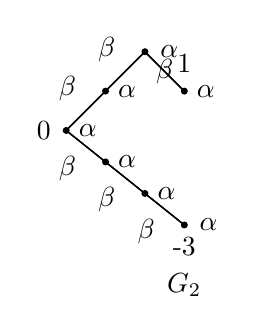
\begin{tikzpicture}
  \draw[line width=0.5pt, rounded corners=8pt, black] 
          (0,0) -- (1.5,-1.2);
  \draw[line width =0.5pt,black]
          (0,0) -- (1,1);
  \draw[line width =0.5pt,black]
          (1,1) -- (1.5,0.5);
  \draw[fill=black, draw=black, line width=0.5pt] (0,0) node[left=0.2em]{0} node[right=0.1em]{$ \alpha $}  circle (1pt);
  \draw[fill=black, draw=black, line width=0.5pt] (1,1) node[right=0.2em]{$ \alpha $}  circle (1pt);
  
  % \draw[fill=black, draw=black, line width=0.5pt] (0.5,-0.33) circle (1pt);
  \draw[fill=black, draw=black, line width=0.5pt] (1.5,-1.2) node[below=1.4em]{$ G_2 $} node[right=0.2em]{$ \alpha $} node[below=0.1em]{-3} circle (1pt);
  \draw[fill=black, draw=black, line width=0.5pt] (0.5,-0.4) node[right=0.1em]{$ \alpha $}  circle (1pt);
  \draw[fill=black, draw=black, line width=0.5pt] (1,-0.8) node[right=0.1em]{$ \alpha $} circle (1pt);
  \draw[fill=black, draw=black, line width=0.5pt] (0.5,0.5) node[right=0.1em]{$ \alpha $}  circle (1pt);
  \draw[fill=black, draw=black, line width=0.5pt] (1.5,0.5) node[right=0.1em]{$ \alpha $} node[above=0.3em]{1} circle (1pt);

  \draw[line width=0.5pt, rounded corners=8pt, black] 
      (0,0) -- node[midway,above left] {$\beta$} (0.5,0.5);
  \draw[line width=0.5pt, rounded corners=8pt, black] 
  (0,0) -- node[midway,below left] {$\beta$} (0.5,-0.4);
  \draw[line width=0.5pt, rounded corners=8pt, black] 
  (0.5,0.5) -- node[midway,above left] {$\beta$} (1,1);
  \draw[line width=0.5pt, rounded corners=8pt, black] 
      (1,1) -- node[midway] {$\beta$} (1.5,0.5);
  \draw[line width=0.5pt, rounded corners=8pt, black] 
      (0.5,-0.4) -- node[midway,below left] {$\beta$} (1,-0.8);
  \draw[line width=0.5pt, rounded corners=8pt, black] 
      (1,-0.8) -- node[midway,below left] {$\beta$} (1.5,-1.2);
\end{tikzpicture}
%图3
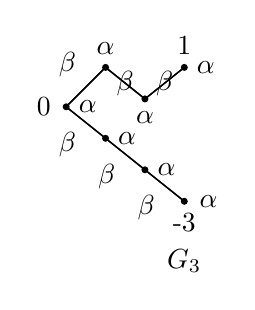
\begin{tikzpicture}
  \draw[line width=0.5pt, rounded corners=8pt, black] 
          (0,0) -- (1.5,-1.2);
  \draw[line width =0.5pt,black]
          (0,0) -- (0.5,0.5);
  \draw[line width =0.5pt,black]
          (0.5,0.5) -- (1,0.1);
  \draw[line width =0.5pt,black]
          (1,0.1) -- (1.5,0.5);
  \draw[fill=black, draw=black, line width=0.5pt] (0,0) node[left=0.2em]{0} node[right=0.1em]{$ \alpha $}  circle (1pt);
  \draw[fill=black, draw=black, line width=0.5pt] (1,0.1) node[below=0.1em]{$ \alpha $} circle (1pt);
  
  % \draw[fill=black, draw=black, line width=0.5pt] (0.5,-0.33) circle (1pt);
  \draw[fill=black, draw=black, line width=0.5pt] (1.5,-1.2) node[below=1.4em]{$ G_3 $} node[right=0.2em]{$ \alpha $} node[below=0.1em]{-3} circle (1pt);
  \draw[fill=black, draw=black, line width=0.5pt] (0.5,-0.4) node[right=0.1em]{$ \alpha $}  circle (1pt);
  \draw[fill=black, draw=black, line width=0.5pt] (1,-0.8) node[right=0.1em]{$ \alpha $} circle (1pt);
  \draw[fill=black, draw=black, line width=0.5pt] (0.5,0.5) node[above=0.1em]{$ \alpha $}  circle (1pt);
  \draw[fill=black, draw=black, line width=0.5pt] (1.5,0.5) node[above=0.1em]{1} node[right=0.1em]{$ \alpha $}   circle (1pt);

  \draw[line width=0.5pt, rounded corners=8pt, black] 
      (0,0) -- node[midway,above left] {$\beta$} (0.5,0.5);
  \draw[line width=0.5pt, rounded corners=8pt, black] 
  (0,0) -- node[midway,below left] {$\beta$} (0.5,-0.4);
  \draw[line width=0.5pt, rounded corners=8pt, black] 
  (0.5,0.5) -- node[midway] {$\beta$} (1,0.1);
  \draw[line width=0.5pt, rounded corners=8pt, black] 
      (1,0.1) -- node[midway] {$\beta$} (1.5,0.5);
  \draw[line width=0.5pt, rounded corners=8pt, black] 
      (0.5,-0.4) -- node[midway,below left] {$\beta$} (1,-0.8);
  \draw[line width=0.5pt, rounded corners=8pt, black] 
      (1,-0.8) -- node[midway,below left] {$\beta$} (1.5,-1.2);

\end{tikzpicture}
%图4
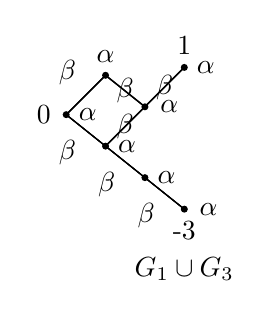
\begin{tikzpicture}
   \draw[line width=0.5pt, rounded corners=8pt, black] 
          (0,0) -- (1.5,-1.2);
  \draw[line width =0.5pt,black]
          (0,0) -- (0.5,0.5);
  \draw[line width =0.5pt,black]
          (0.5,0.5) -- (1,0.1);
  \draw[line width =0.5pt,black]
          (1,0.1) -- (1.5,0.6);
    \draw[line width =0.5pt,black]
          (0.5,-0.4) -- (1,0.1);
  \draw[fill=black, draw=black, line width=0.5pt] (0,0) node[left=0.2em]{0} node[right=0.1em]{$ \alpha $}  circle (1pt);
  \draw[fill=black, draw=black, line width=0.5pt] (1,0.1) node[right=0.2em]{$ \alpha $} circle (1pt);
  
  % \draw[fill=black, draw=black, line width=0.5pt] (0.5,-0.33) circle (1pt);
  \draw[fill=black, draw=black, line width=0.5pt] (1.5,-1.2) node[below=1.4em]{$ G_1 \cup G_3 $} node[right=0.2em]{$ \alpha $} node[below=0.1em]{-3} circle (1pt);
  \draw[fill=black, draw=black, line width=0.5pt] (0.5,-0.4) node[right=0.1em]{$ \alpha $}  circle (1pt);
  \draw[fill=black, draw=black, line width=0.5pt] (1,-0.8) node[right=0.1em]{$ \alpha $} circle (1pt);
  \draw[fill=black, draw=black, line width=0.5pt] (0.5,0.5) node[above=0.1em]{$ \alpha $}  circle (1pt);
  \draw[fill=black, draw=black, line width=0.5pt] (1.5,0.6) node[above=0.1em]{1} node[right=0.1em]{$ \alpha $}   circle (1pt);

 \draw[line width=0.5pt, rounded corners=8pt, black] 
      (0,0) -- node[midway,above left] {$\beta$} (0.5,0.5);
  \draw[line width=0.5pt, rounded corners=8pt, black] 
  (0,0) -- node[midway,below left] {$\beta$} (0.5,-0.4);
  \draw[line width=0.5pt, rounded corners=8pt, black] 
  (0.5,0.5) -- node[midway] {$\beta$} (1,0.1);
  \draw[line width=0.5pt, rounded corners=8pt, black] 
      (1,0.1) -- node[midway] {$\beta$} (1.5,0.6);
  \draw[line width=0.5pt, rounded corners=8pt, black] 
      (0.5,-0.4) -- node[midway,below left] {$\beta$} (1,-0.8);
  \draw[line width=0.5pt, rounded corners=8pt, black] 
      (1,-0.8) -- node[midway,below left] {$\beta$} (1.5,-1.2);
  \draw[line width=0.5pt, rounded corners=8pt, black] 
      (0.5,-0.4) -- node[midway] {$\beta$} (1,0.1);

\end{tikzpicture}
\\
\\
%图5
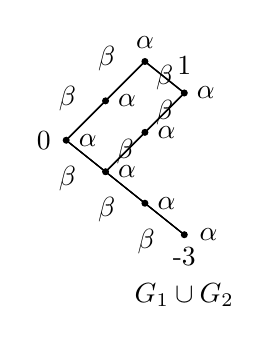
\begin{tikzpicture}
  \draw[line width=0.5pt, rounded corners=8pt, black] 
          (0,0) -- (1.5,-1.2);
  \draw[line width =0.5pt,black]
          (0,0) -- (1,1);
  \draw[line width =0.5pt,black]
          (1,1) -- (1.5,0.6);
  \draw[line width =0.5pt,black]
          (0.5,-0.4) -- (1.5,0.6);
  \draw[fill=black, draw=black, line width=0.5pt] (0,0) node[left=0.2em]{0} node[right=0.1em]{$ \alpha $}  circle (1pt);
  \draw[fill=black, draw=black, line width=0.5pt] (1,1) node[above=0.1em]{$ \alpha $} circle (1pt);
  
  % \draw[fill=black, draw=black, line width=0.5pt] (0.5,-0.33) circle (1pt);
  \draw[fill=black, draw=black, line width=0.5pt] (1.5,-1.2) node[below=1.4em]{$ G_1\cup G_2 $} node[right=0.2em]{$ \alpha $} node[below=0.1em]{-3} circle (1pt);
  \draw[fill=black, draw=black, line width=0.5pt] (0.5,-0.4) node[right=0.1em]{$ \alpha $}  circle (1pt);
  \draw[fill=black, draw=black, line width=0.5pt] (1,-0.8) node[right=0.1em]{$ \alpha $} circle (1pt);
  \draw[fill=black, draw=black, line width=0.5pt] (0.5,0.5) node[right=0.1em]{$ \alpha $}  circle (1pt);
  \draw[fill=black, draw=black, line width=0.5pt] (1.5,0.6) node[right=0.1em]{$ \alpha $}  node[above=0.3em]{1}   circle (1pt);
  \draw[fill=black, draw=black, line width=0.5pt] (1,0.1) node[right=0.1em]{$ \alpha $}  circle (1pt);

  \draw[line width=0.5pt, rounded corners=8pt, black] 
      (0,0) -- node[midway,above left] {$\beta$} (0.5,0.5);
  \draw[line width=0.5pt, rounded corners=8pt, black] 
  (0,0) -- node[midway,below left] {$\beta$} (0.5,-0.4);
  \draw[line width=0.5pt, rounded corners=8pt, black] 
  (0.5,0.5) -- node[midway,above left] {$\beta$} (1,1);
  \draw[line width=0.5pt, rounded corners=8pt, black] 
      (1,1) -- node[midway] {$\beta$} (1.5,0.6);
  \draw[line width=0.5pt, rounded corners=8pt, black] 
      (0.5,-0.4) -- node[midway,below left] {$\beta$} (1,-0.8);
  \draw[line width=0.5pt, rounded corners=8pt, black] 
      (1,-0.8) -- node[midway,below left] {$\beta$} (1.5,-1.2);
  \draw[line width=0.5pt, rounded corners=8pt, black] 
      (0.5,-0.4) -- node[midway] {$\beta$} (1,0.1);
 \draw[line width=0.5pt, rounded corners=8pt, black] 
      (1,0.1) -- node[midway] {$\beta$} (1.5,0.6);

\end{tikzpicture}
%图6
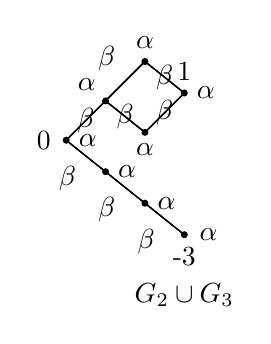
\begin{tikzpicture}
  \draw[line width=0.5pt, rounded corners=8pt, black] 
          (0,0) -- (1.5,-1.2);
  \draw[line width =0.5pt,black]
          (0,0) -- (0.5,0.5);
  \draw[line width =0.5pt,black]
          (0.5,0.5) -- (1,1);
  \draw[line width =0.5pt,black]
          (1,0.1) -- (1.5,0.6);
  \draw[line width =0.5pt,black]
          (0.5,0.5) -- (1,1);
  \draw[line width =0.5pt,black]
          (1,1) -- (1.5,0.6);
  \draw[line width =0.5pt,black]
          (0.5,0.5) -- (1,0.1);
  \draw[fill=black, draw=black, line width=0.5pt] (0,0) node[left=0.2em]{0} node[right=0.1em]{$ \alpha $}  circle (1pt);
  \draw[fill=black, draw=black, line width=0.5pt] (1,0.1) node[below=0.05em]{$ \alpha $} circle (1pt);
  
  % \draw[fill=black, draw=black, line width=0.5pt] (0.5,-0.33) circle (1pt);
  \draw[fill=black, draw=black, line width=0.5pt] (1.5,-1.2) node[below=1.4em]{$ G_2\cup G_3 $} node[right=0.2em]{$ \alpha $} node[below=0.1em]{-3} circle (1pt);
  \draw[fill=black, draw=black, line width=0.5pt] (0.5,-0.4) node[right=0.1em]{$ \alpha $}  circle (1pt);
  \draw[fill=black, draw=black, line width=0.5pt] (1,-0.8) node[right=0.1em]{$ \alpha $} circle (1pt);
  \draw[fill=black, draw=black, line width=0.5pt] (0.5,0.5) node[above left]{$ \alpha $}  circle (1pt);
  \draw[fill=black, draw=black, line width=0.5pt] (1.5,0.6) node[above=0.1em]{1} node[right=0.1em]{$ \alpha $}   circle (1pt);
  \draw[fill=black, draw=black, line width=0.5pt] (1,1) node[above=0.1em]{$ \alpha $}  circle (1pt);


  \draw[line width=0.5pt, rounded corners=8pt, black] 
      (0,0) -- node[midway] {$\beta$} (0.5,0.5);
  \draw[line width=0.5pt, rounded corners=8pt, black] 
  (0,0) -- node[midway,below left] {$\beta$} (0.5,-0.4);
  \draw[line width=0.5pt, rounded corners=8pt, black] 
  (0.5,0.5) -- node[midway] {$\beta$} (1,0.1);
  \draw[line width=0.5pt, rounded corners=8pt, black] 
      (1,0.1) -- node[midway] {$\beta$} (1.5,0.6);
  \draw[line width=0.5pt, rounded corners=8pt, black] 
      (0.5,-0.4) -- node[midway,below left] {$\beta$} (1,-0.8);
  \draw[line width=0.5pt, rounded corners=8pt, black] 
      (1,-0.8) -- node[midway,below left] {$\beta$} (1.5,-1.2);
  \draw[line width=0.5pt, rounded corners=8pt, black] 
      (0.5,0.5) -- node[midway,above left] {$\beta$} (1,1);
  \draw[line width=0.5pt, rounded corners=8pt, black] 
      (1,1) -- node[midway] {$\beta$} (1.5,0.6);

\end{tikzpicture}
%图7
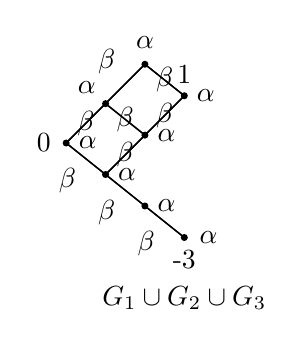
\begin{tikzpicture}
  \draw[line width=0.5pt, rounded corners=8pt, black] 
          (0,0) -- (1.5,-1.2);
  \draw[line width =0.5pt,black]
          (0,0) -- (1,1);
  \draw[line width =0.5pt,black]
          (1,1) -- (1.5,0.6);
  \draw[line width =0.5pt,black]
          (0.5,-0.4) -- (1.5,0.6);
  \draw[line width =0.5pt,black]
          (0.5,0.5) -- (1,0.1);        
  \draw[fill=black, draw=black, line width=0.5pt] (0,0) node[left=0.2em]{0} node[right=0.1em]{$ \alpha $}  circle (1pt);

  \draw[fill=black, draw=black, line width=0.5pt] (1,1) node[above=0.2em]{$ \alpha $} circle (1pt);
  
  % \draw[fill=black, draw=black, line width=0.5pt] (0.5,-0.33) circle (1pt);
  \draw[fill=black, draw=black, line width=0.5pt] (1.5,-1.2) node[below=1.4em]{$ G_1\cup G_2\cup G_3 $} node[right=0.2em]{$ \alpha $} node[below=0.1em]{-3} circle (1pt);
  \draw[fill=black, draw=black, line width=0.5pt] (0.5,-0.4) node[right=0.1em]{$ \alpha $}  circle (1pt);
  \draw[fill=black, draw=black, line width=0.5pt] (1,-0.8) node[right=0.1em]{$ \alpha $} circle (1pt);
  \draw[fill=black, draw=black, line width=0.5pt] (0.5,0.5) node[above left]{$ \alpha $}  circle (1pt);
  \draw[fill=black, draw=black, line width=0.5pt] (1.5,0.6) node[right=0.1em]{$ \alpha $} node[above=0.1em]{1}   circle (1pt);
  \draw[fill=black, draw=black, line width=0.5pt] (1,0.1) node[right=0.1em]{$ \alpha $}  circle (1pt);

  \draw[line width=0.5pt, rounded corners=8pt, black] 
      (0,0) -- node[midway] {$\beta$} (0.5,0.5);
  \draw[line width=0.5pt, rounded corners=8pt, black] 
  (0,0) -- node[midway,below left] {$\beta$} (0.5,-0.4);
  \draw[line width=0.5pt, rounded corners=8pt, black] 
  (0.5,0.5) -- node[midway] {$\beta$} (1,0.1);
  \draw[line width=0.5pt, rounded corners=8pt, black] 
      (1,0.1) -- node[midway] {$\beta$} (1.5,0.6);
  \draw[line width=0.5pt, rounded corners=8pt, black] 
      (0.5,-0.4) -- node[midway,below left] {$\beta$} (1,-0.8);
  \draw[line width=0.5pt, rounded corners=8pt, black] 
      (1,-0.8) -- node[midway,below left] {$\beta$} (1.5,-1.2);
  \draw[line width=0.5pt, rounded corners=8pt, black] 
      (0.5,0.5) -- node[midway,above left] {$\beta$} (1,1);
  \draw[line width=0.5pt, rounded corners=8pt, black] 
      (1,1) -- node[midway] {$\beta$} (1.5,0.6);
  \draw[line width=0.5pt, rounded corners=8pt, black] 
      (0.5,-0.4) -- node[midway] {$\beta$} (1,0.1);


\end{tikzpicture}
\end{figure}
\ \\
しがたって、\\


\begin{align*}
  \sigma_3 \left(\left\{0\right\}, \left\{-3,1\right\}\right) &= \alpha^{-1} W_3 \left(\left\{0\right\},\left\{-3,1\right\}\right)\\ \notag
  &= \alpha^{-1}\left\{w_3(G_1)+w_3(G_2)+w_3(G_3)+w_3(G_1\cup G_3)+w_3(G_1\cup G_2)+w_3(G_2\cup G_3)+w_3(G_1\cup G_2\cup G_3)\right\} \\ \notag
  &= \alpha^{-1}\left\{\alpha^6 \beta^5+\alpha^7\beta^6+\alpha^7\beta^6+(-1)\alpha^7 \beta^7+(-1)\alpha^8 \beta^8+(-1)\alpha^8 \beta^8+(-1)^2\alpha^8 \beta^9\right\} \\ \notag
  &=(\alpha \beta)^5+2(\alpha \beta)^6-(\alpha \beta)^5(p \beta)-2(\alpha \beta)^6(p \beta)+(\alpha \beta)^5(p \beta)^2 \\ \notag
  &=p^5+2p^6-p^5(2p-q)-2p^6(2p-q)+p^5(2p-q)^2 \\ \notag
  &=p^5\left(1+q-2pq+q^2\right)\\ \notag
\end{align*}
ここで、 $ \alpha \beta=p $,\  $ \alpha \beta^2 =p \beta=2p-q $を用いた\\

\end{proof}
\end{document}



